\documentclass[a4paper,12pt,titlepage,finall]{article}

\usepackage{fancyvrb}
\usepackage{amsmath}
\usepackage{float}
\usepackage[T1,T2A]{fontenc}     % форматы шрифтов
\usepackage[utf8x]{inputenc}     % кодировка символов, используемая в данном файле
\usepackage[russian]{babel}      % пакет русификации
\usepackage{tikz}                % для создания иллюстраций
\usepackage{pgfplots}            % для вывода графиков функций
\usepackage{geometry}		 % для настройки размера полей
\usepackage{indentfirst}         % для отступа в первом абзаце секции
\usepackage{listings}

% выбираем размер листа А4, все поля ставим по 3см
\geometry{a4paper,left=30mm,top=30mm,bottom=30mm,right=30mm}

\setcounter{secnumdepth}{0}      % отключаем нумерацию секций

\usepgfplotslibrary{fillbetween} % для изображения областей на графиках

\begin{document}
\begin{titlepage}
  \begin{center}
      \begin{minipage}{0.10\textwidth}%
          
\includegraphics[width=0.8\textwidth]{msu-logo2.png}%
      \end{minipage}\hspace{10pt}
      \begin{minipage}{0.7\textwidth}%
        \small\bf\centering
        МОСКОВСКИЙ~ГОСУДАРСТВЕННЫЙ~УНИВЕРСИТЕТ\\
        имени~M.~В.~Ломоносова\\
        ~\\
        Факультет вычислительной математики и кибернетики
      \end{minipage}\hspace{10pt}
      \begin{minipage}{0.10\textwidth}%
          
\includegraphics[width=0.8\textwidth]{cmc-logo.png}%
      \end{minipage}\\
      ~\\
      \par\noindent\rule{\textwidth}{0.1pt}
    \vfill
    ~\\
    {\large \bf
      Практикум по учебному курсу\\
      <<Распределенные системы>>\\
    }
    ~\\
    ~\\
    {\large \bf
      Отчет\\
      о выполненном задании
    }\\
    {\large
      студента 427 учебной группы факультета ВМК МГУ
    }\\
    ~\\
    {\small
      Кобрина Илая Александровича
      \begin{center}
      \end{center}
    }
  \end{center}
  \begin{center}
    \vfill
    {\small Москва\\2022}
  \end{center}
\end{titlepage}

%\tableofcontents
%\newpage

%\section{

% Автоматически генерируем оглавление на отдельной странице
\tableofcontents
\newpage
\section{Задание 1}
\subsection{Постановка задачи}
В транспьютерной матрице размером 4*4, в каждом узле которой находится один
процесс, необходимо выполнить операцию рассылки данных всем процессам от одного
(MPI\_SCATTERV) --- от процесса с координатами (0,0). Каждый i-ый процесс должен получить i чисел (длинной 4 байта).

Реализовать программу, моделирующую выполнение операции MPI\_SCATTERV на транспьютерной матрице при помощи пересылок MPI типа точка-точка.
Получить временную оценку работы алгоритма. Оценить сколько времени потребуется
для выполнения операции MPI\_SCATTERV, если все процессы выдали ее одновременно. Время старта равно 100, время передачи байта равно 1 (Ts=100,Tb=1). Процессорные операции, включая чтение из памяти и запись в память, считаются бесконечно быстрыми.
\subsection{Описание алгоритма}

Пересылка сообщений организована следующим образом:
\begin{center}
    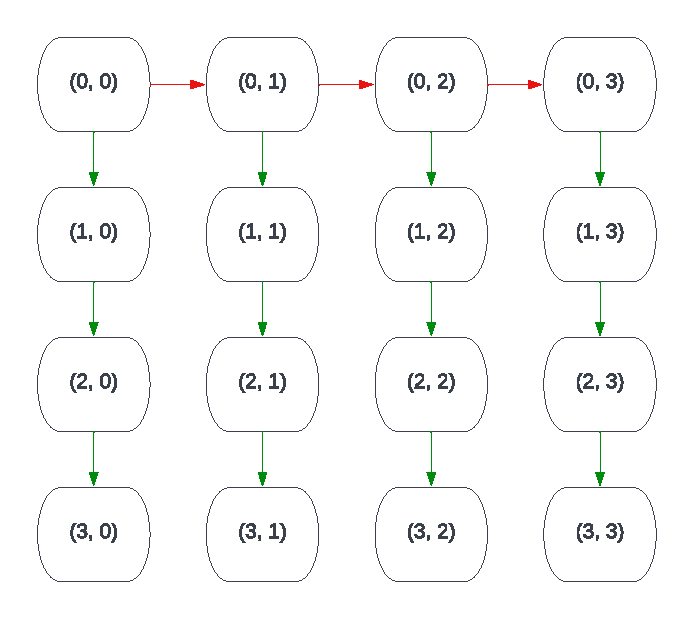
\includegraphics[scale=1.5, width=\linewidth]{p_matrix.pdf}
\end{center}

В начале процесс (0, 0) посылает все сообщения, адресатами которых являются
процессы, не находящиеся в его столбце, вправо по нулевой строке. Как только сообщение
доходит до процесса в нулевой строке, находящимся в одном столбце с адресатом
сообщения, он посылает сообщение далее по своему столбцу, пока оно не дойдет до
своего адресата. Если процессу в нулевой строке пришло сообщение для процесса не
из его столбца, процесс посылает сообщение далее по нулевой строк вправо.

Так как каждый процесс должен получить соответствующее его номеру количество
чисел по 4 байт, процессы должны заранее знать, какого размера буфер им
необходимо принимать на вход. Это реализовано благодаря служебным сообщениям.
Перед тем как отправлять сообщение, процессы отправляют служебное сообщение,
содержащее число размером 4 байта, соответствующее номеру адресата (и количеству
байтов для буфера, соответственно). Далее принимающий процесс выделяет буфер
нужного размера и принимает соответствующую последовательность чисел.

Процесс завершает свою работу, как только он принимает свои собственные i чисел.
Таким образом, начиная отправлять сообщения с 15-го по 1-й, каждый процесс
получит свое сообщение.

\subsection{Оценка времени работы алгоритма}

Сообщение для 4-го, 8-го и 12-го процессов будут отправлены 1, 2 и 3 раза
соответственно: $T_4 + T_8 + T_{12} = (T_s + 4 * T_b * 4) + 2 * (T_s + 4 * T_b * 8) +
3 * (T_s + 4 * T_b * 12) = 6T_s + 224T_b$.

Сообщение для 5-го, 9-го и 13-го процессов будут отправлены 2, 3 и 4 раза
соответственно: $T_5 + T_9 + T_{13} = 2 * (T_s + 4 * T_b * 5) + 3 * (T_s + 4 * T_b
* 9) + 4 * (T_s + 4 * T_b * 13) = 9T_s + 356T_b$.

Сообщение для 6-го, 10-го и 14-го процессов будут отправлены 3, 4 и 5 раза
соответственно: $T_6 + T_{10} + T_{14} = 3 * (T_s + 4 * T_b * 6) + 4 * (T_s + 4 * T_b
* 10) + 5 * (T_s + 4 * T_b * 14) = 12T_s + 512T_b$.

Сообщение для 7-го, 11-го и 15-го процессов будут отправлены 4, 5 и 6 раза
соответственно: $T_7 + T_{11} + T_{15} = 4 * (T_s + 4 * T_b * 7) + 5 * (T_s + 4 * T_b
* 11) + 6 * (T_s + 4 * T_b * 15) = 15T_s + 692T_b$.

Сообщение для 1-го, 2-го и 3-го процессов будут отправлены 1, 2 и 3 раза
соответственно: $T_1 + T_2 + T_3 = (T_s + 4 * T_b * 1) + 2 * (T_s + 4 * T_b * 2)
+ 3 * (T_s + 4 * T_b * 3) = 6T_s + 56T_b$.

Также для отправки всех этих сообщений было отправлено 48 служебных сообщений по
4 байта каждое:
$T_add = 48 * (T_s + 4 * T_b) = 48T_s + 192T_b$.

Итого, $T = 96T_s + 2032T_b = 11632$

\subsection{Работа программы}

Для запуска программы необходимо её скомпилировать и запустить:

\begin{lstlisting}
mpic++ -o scatterv scatterv.cpp
mpirun --oversubscribe -np 16 scatterv
\end{lstlisting}

При удачном завершении работы, нулевой процесс должен сообщить о том, что
отправил все сообщения, и завершиться, а каждый i-й процесс должен вывести
полученные им i чисел от 1 до i соответственно, после чего также завершиться.

\newpage

\section{Задание 2}
\subsection{Постановка задачи}

Доработать MPI-программу, реализованную в рамках курса
“Суперкомпьютеры и параллельная обработка данных” - FDTD-2D. Добавить
контрольные точки для продолжения работы программы в случае сбоя. Реализовать
один из 3-х сценариев работы после сбоя: a) продолжить работу программы только
на “исправных” процессах; б) вместо процессов, вышедших из строя, создать новые
MPI-процессы, которые необходимо использовать для продолжения расчетов; в) при
запуске программы на счет сразу запустить некоторое дополнительное количество
MPI-процессов, которые использовать в случае сбоя.

\subsection{Описание алгоритма}

Был выбран третий вариант -- создание резервных процессов в начале работы
программы. В начале работы
программы для глобального коммуникатора создается обработчик ошибок, а также
с помощью макроса \texttt{HELPERS} задается количество вспомогательных
процессов. Далее для всех активных процессов инициализируются матрицы и
распределяется работа. Затем начинаются вычисления, во время которых резервные
процессы просто простаивают. Каждые 5 итераций текущие результаты вычислений
сохраняются на диск; также сохраняется на диск номер текущей итерации. Когда
один из процессов падает, все процессы, включая резервные, попадают в
обработчик, где выясняется количество упавших процессов и обновляется
коммуникатор. Далее процессам заново назначаются номера и для каждого процесса
реаллоцируются буферы для вычислений (для резервного процесса аллоцируются
впервые), а последнее сохраненное состояние вычислений грузится с диска.

Если количество упавших процессов больше количества оставшихся резервных
процессов, работа программы завершается при помощи \texttt{MPI\_Abort}.

Если при падении состояние вычислений еще ни разу не сохранялось на диск, работа
начинается с самого начала, как если бы программу только что запустили.

\subsection{Работа программы}

Для запуска программы необходимо её скомпилировать и запустить:

\begin{lstlisting}
mkdir run && cd run
mpicc -g -o fdtd ../fdtd-2d.c
mpirun -v -np 11 --enable-recovery --with-ft=ulfm --oversubscribe fdtd
\end{lstlisting}

\end{document}
